\documentclass[dvipdfmx]{jsarticle}


\usepackage{tcolorbox}
\usepackage{color}
\usepackage{listings, plistings}

%% ノート/latexメモ
%% http://pepper.is.sci.toho-u.ac.jp/pepper/index.php?%A5%CE%A1%BC%A5%C8%2Flatex%A5%E1%A5%E2

%% JavaScriptの設定
%% https://e8l.hatenablog.com/entry/2015/11/29/232800
\lstdefinelanguage{javascript}{
  morekeywords = [1]{ %keywords
    await, break, case, catch, class, const, continue, debugger, default, delete, 
    do, else, enum, export, extends, finally, for, function, function*, if, implements, import, in, 
    instanceof, interface, let, new, package, private, protected, public, return, static, super,
    switch, this, throw, try, typeof, var, void, while, with, yield, yield*
  },
  morekeywords = [2]{ %literal
    false, Infinity, NaN, null, true, undefined
  },
  morekeywords = [3] { %Classes
    Array, ArrayBuffer, Boolean, DataView, Date, Error, EvalError, Float32Array, Float64Array,
    Function, Generator, GeneratorFunction, Int16Array, Int32Array, Int8Array, InternalError,
    JSON, Map, Math, Number, Object, Promise, Proxy, RangeError, ReferenceError, Reflect,
    RegExp, Set, String, Symbol, SyntaxError, TypeError, URIError, Uint16Array, Uint32Array,
    Uint8Array, Uint8ClampedArray, WeakMap, WeakSet
  },
  morecomment = [l]{//},
  morecomment = [s]{/*}{*/},
  morestring = [b]{"},
  morestring = [b]{'},
  alsodigit = {-},
  sensitive = true
}

%% 修正時刻: Tue 2022/03/15 10:04:41


% Java
\lstset{% 
  frame=single,
  backgroundcolor={\color[gray]{.9}},
  stringstyle={\ttfamily \color[rgb]{0,0,1}},
  commentstyle={\itshape \color[cmyk]{1,0,1,0}},
  identifierstyle={\ttfamily}, 
  keywordstyle={\ttfamily \color[cmyk]{0,1,0,0}},
  basicstyle={\ttfamily},
  breaklines=true,
  xleftmargin=0zw,
  xrightmargin=0zw,
  framerule=.2pt,
  columns=[l]{fullflexible},
  numbers=left,
  stepnumber=1,
  numberstyle={\scriptsize},
  numbersep=1em,
  language={Java},
  lineskip=-0.5zw,
  morecomment={[s][{\color[cmyk]{1,0,0,0}}]{/**}{*/}},
  keepspaces=true,         % 空白の連続をそのままで
  showstringspaces=false,  % 空白字をOFF
}
%\usepackage[dvipdfmx]{graphicx}
\usepackage{url}
\usepackage[dvipdfmx]{hyperref}
\usepackage{amsmath, amssymb}
\usepackage{itembkbx}
\usepackage{eclbkbox}	% required for `\breakbox' (yatex added)
\usepackage{enumerate}
\usepackage[default]{cantarell}
\usepackage[T1]{fontenc}
\fboxrule=0.5pt
\parindent=1em
\definecolor{mygrey}{rgb}{0.97, 0.97, 0.97}

\makeatletter
\def\verbatim@font{\normalfont
\let\do\do@noligs
\verbatim@nolig@list}
\makeatother

\begin{document}

%\anaumeと入力すると穴埋め解答欄が作れるようにしてる。\anaumesmallで小さめの穴埋めになる。
\newcounter{mycounter} % カウンターを作る
\setcounter{mycounter}{0} % カウンターを初期化
\newcommand{\anaume}[1][]{\refstepcounter{mycounter}{#1}{\boxed{\phantom{aa}\textnormal{\themycounter}\phantom{aa}}}} %穴埋め問題の空欄作ってる。
\newcommand{\anaumesmall}[1][]{\refstepcounter{mycounter}{#1}{\boxed{\tiny{\phantom{a}\themycounter \phantom{a}}}}}%小さい版作ってる。色々改造できる。

%% 修正時刻: Tue 2022/03/15 10:04:411


\newpage

\section{XAMPPの設定}

\subsection{TeraPad の登録}

''XAMPPコントロールパネル'' が起動したら、まず、右上の ``Config'' をクリックする。

\vspace{3mm}
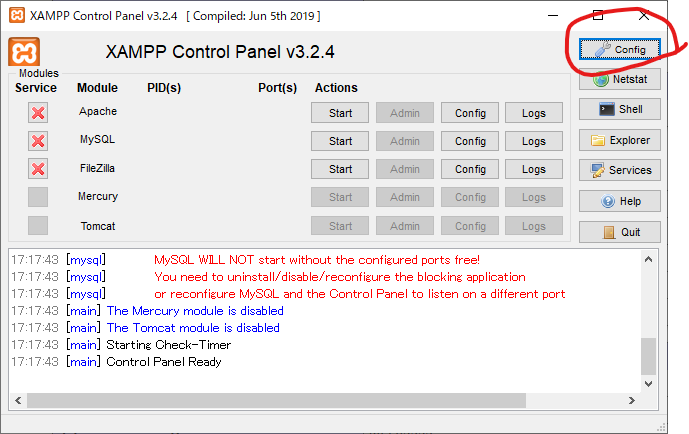
\includegraphics[width=12cm]{../03-config/21-config.png}
\vspace{3mm}

次に開いた窓で、''Editor'' の設定を変更する。

メモ帳 が初期値になっているので、それを ``TeraPad'' に変更する。

\textsf{C:\yen Program Files (x86)\yen terapad\yen TeraPad.exe} を指定する。

\vspace{3mm}
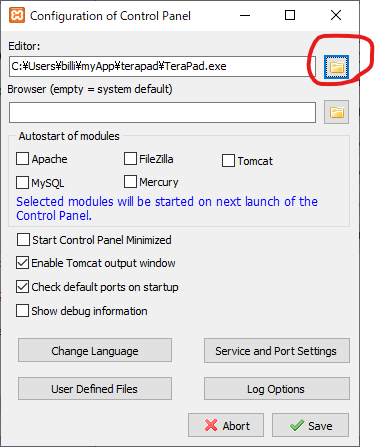
\includegraphics[width=10cm]{../03-config/22-terapad.png}
\vspace{3mm}

\newpage
\subsection{php.ini の設定}

XAMPPコントロールパネルの ''Apache'' の行の ``Config'' をクリックして、
表示されたサブメニューから \textsf{PHP (pho.ini)} を選択する。

\vspace{3mm}
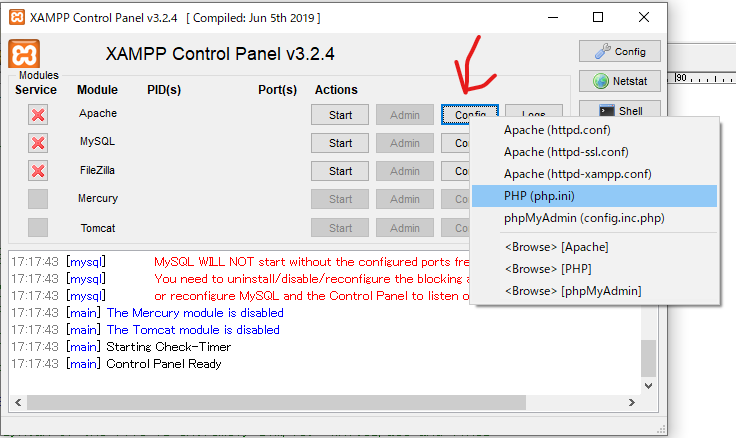
\includegraphics[width=14cm]{../04-php-ini/11-php-ini.png}
\vspace{3mm}

php.ini が TeraPad で 開くので、上の虫メガネの左端のアイコンをクリックして、
出てきたウィンドウで、\textsf{timezone} と入力して、 ``先頭から検索'' を
クリックする。

\vspace{3mm}
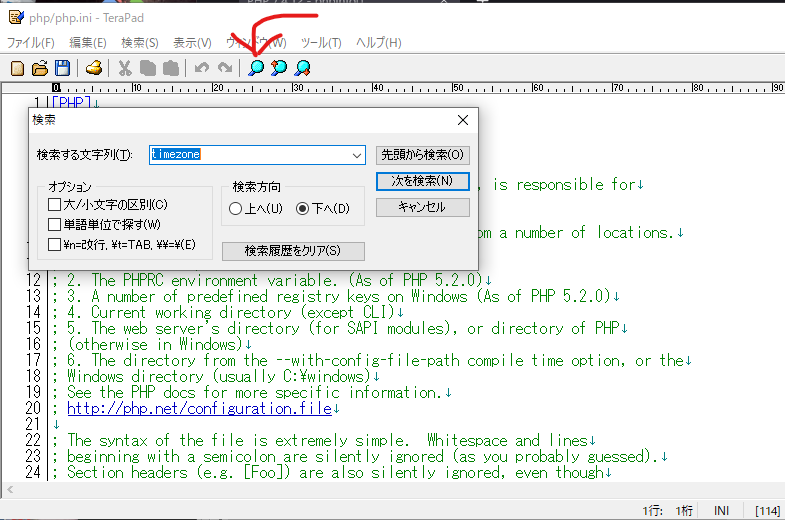
\includegraphics[width=13cm]{../04-php-ini/12-timezone.png}
\vspace{3mm}

上の虫メガネの右端のアイコンを 2回 あるいは 3回 クリックすると、
1972行目あたりに \textsf{date.timezone=Europe/Berlin} という行が
見つかる。

\vspace{3mm}
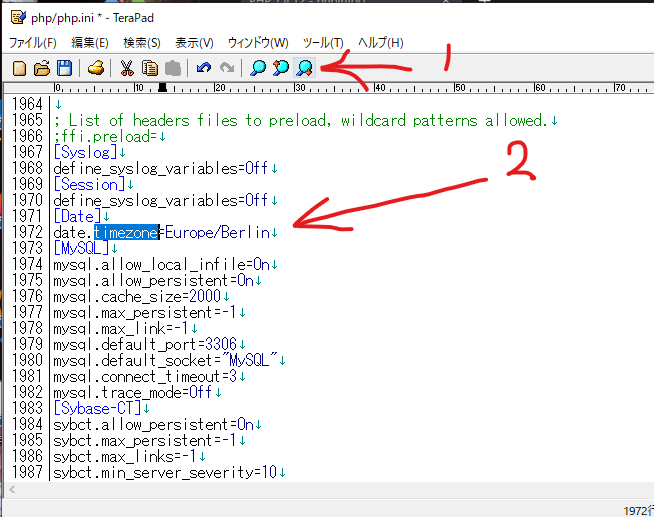
\includegraphics[width=13cm]{../04-php-ini/13-find-timezone.png}
\vspace{3mm}


その Europe/Berlin を \textsf{Asia/Tokyo} に変更する。

\vspace{3mm}
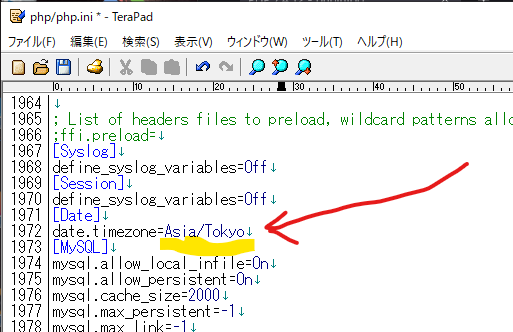
\includegraphics[width=13cm]{../04-php-ini/14-asia-tokyo.png}
\vspace{3mm}

これで、php.ini の設定は終了である。

\subsection{余談 ------ mbstring の設定}

『PHPノート』(p.25)に載っている mbstring の設定は、PHP5.6以降(だったかな)は不要(非推奨)である。
現在では、\textsf{timezone} の設定だけでいける。

\href{https://www.php.net/manual/ja/mbstring.configuration.php}{https://www.php.net/manual/ja/mbstring.configuration.php}

\subsection{my.iniの設定}

XAMPPコントロールパネルの''MySQL''の行の''Config''をクリックして、
表示されたサブメニューから ``my.ini'' を選択する。

\vspace{3mm}
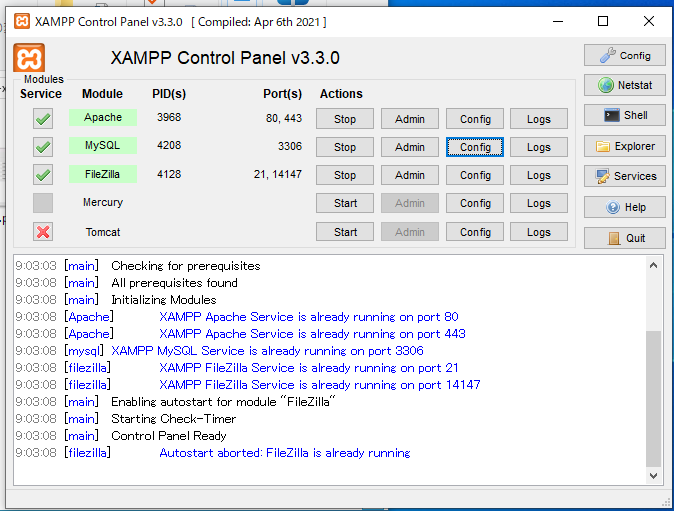
\includegraphics[width=13cm]{img/mysql-config.png}
\vspace{3mm}

my.iniがTeraPadで開くので、

\begin{lstlisting}[numbers=none]
 [client]
 ...
 default-character-set=utf8mb4             # <-
 ...
 [mysqld]
\end{lstlisting}

\vspace{3mm}
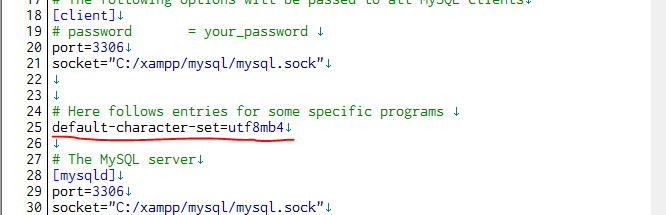
\includegraphics[width=13cm]{img/my-ini-01.png}
\vspace{3mm}


\begin{lstlisting}[numbers=none]
 ...
 [mysqld]
 ...
 character-set-server=utf8mb4               # <-
 collation-server=utf8mb4_general_ci        # <-
 ...
 [mysqldump]
\end{lstlisting}

\vspace{3mm}
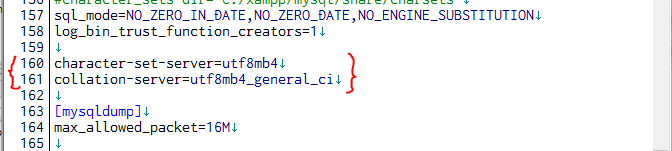
\includegraphics[width=13cm]{img/my-ini-02.png}
\vspace{3mm}

上記のように記述を追加したのち、
mysql を ``stop'' してから ``start'' と再起動する。

\vspace{6mm}
\textgt{確認方法}

コマンドプロンプトを起動して、MySQLにログインする。

\framebox{$>$ mysql -u root -p}

以下のコマンドを実行する。


\begin{tabular}{|l|} \hline
 \verb!MariaDB[(nome)]> show variables like '%char%';! \\ \hline
\end{tabular}

以下のように表示されればよい。

\vspace{3mm}
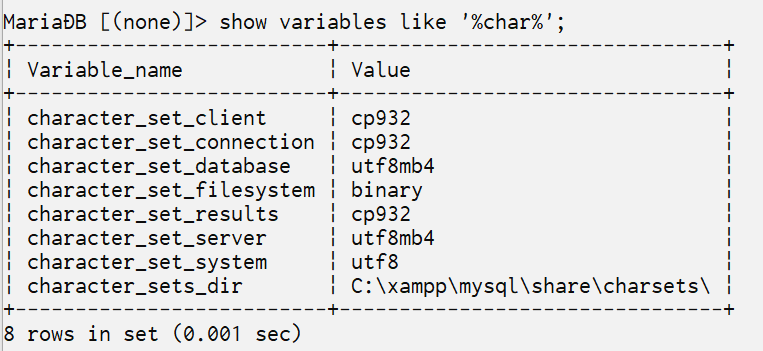
\includegraphics[width=13cm]{img/charset.png}
\vspace{3mm}



\vspace{3cm}

\section{環境変数への登録}

\subsection{php を環境変数 Path に登録する}

\subsubsection{システム環境変数の編集}

システム環境変数の \textsf{PATH} に、php.exe のある場所を登録する。

スタートボタン右の 虫メガネ に、''システム'' と入力し、表示された候補から
''システム環境変数の編集'' を選択する。

\vspace{3mm}
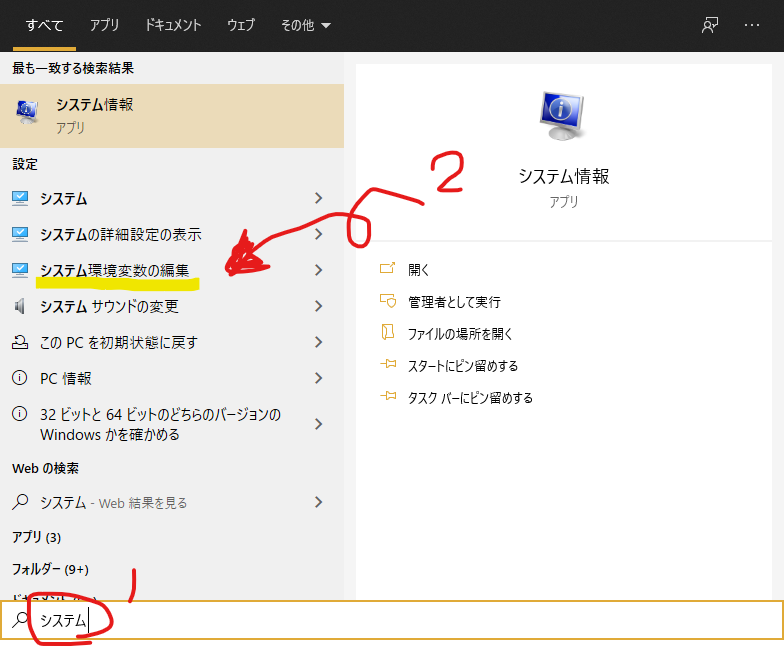
\includegraphics[width=14cm]{../05-path/01-system-variable.png}
\vspace{3mm}

開いたウィンドウで、''環境変数'' をクリックする。

\vspace{3mm}
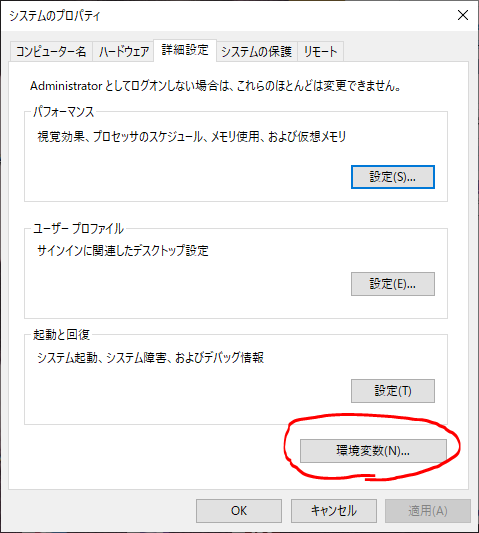
\includegraphics[width=8cm]{../05-path/02-env-variable.png}
\vspace{3mm}

開いたウィンドウで、下の ``システム環境変数'' の ''\textsf{Path}'' を
選択する。

そして、下の ''編集'' をクリックする。

\vspace{3mm}
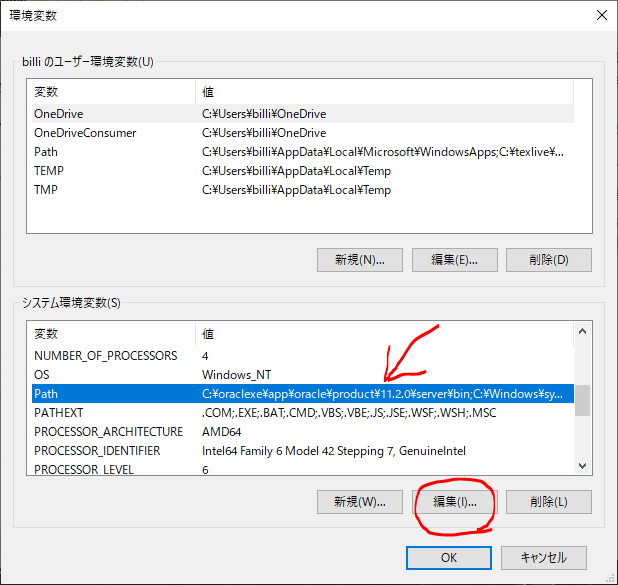
\includegraphics[width=11cm]{../05-path/03-path.png}
\vspace{3mm}

''環境変数名の編集''画面で、''新規'' を選択する。

\vspace{3mm}
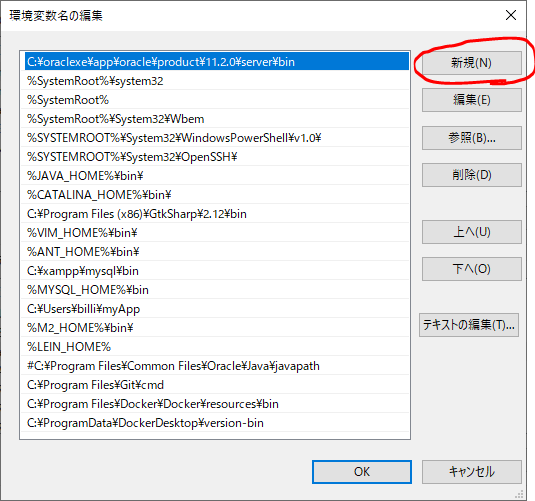
\includegraphics[width=13cm]{../05-path/04-new-path.png}
\vspace{3mm}

空欄の項目ができるので、そこに
\begin{tcolorbox}
 C:\yen xampp\yen php
\end{tcolorbox}

と、入力する。

\vspace{3mm}
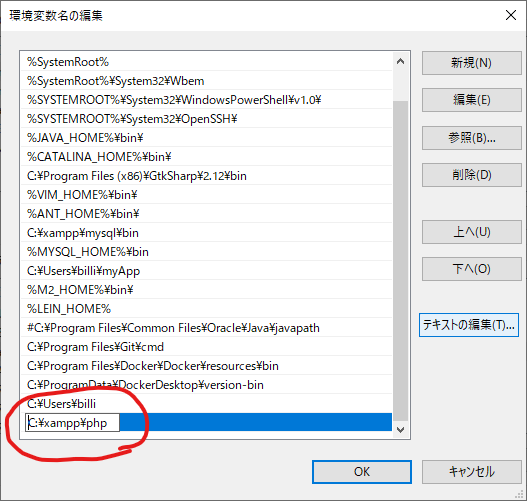
\includegraphics[width=13cm]{../05-path/05-path-xampp-php.png}
\vspace{3mm}

あとは、''OK'' をクリックして閉じていく。
``×'' や ''キャンセル'' をクリックすると、設定が反映されない。
必ず ''OK'' をクリックする。

\subsubsection{確認}

もし、今、コマンドプロンプトの黒い画面が開いていたら、いったん閉じる。

それから、コマンドプロンプトを開いて、以下のコマンドを入力する。

\begin{tcolorbox}
 $>$ php -v
\end{tcolorbox}

PHPのバージョンが表示されれば成功である。

\newpage

\subsection{mysql を環境変数 Path に登録する}

phpのときと同様にして、mysql を環境変数 Path に登録する。

登録するパスは \textsf{C:\yen xampp\yen mysql\yen bin} である。

\vspace{3mm}
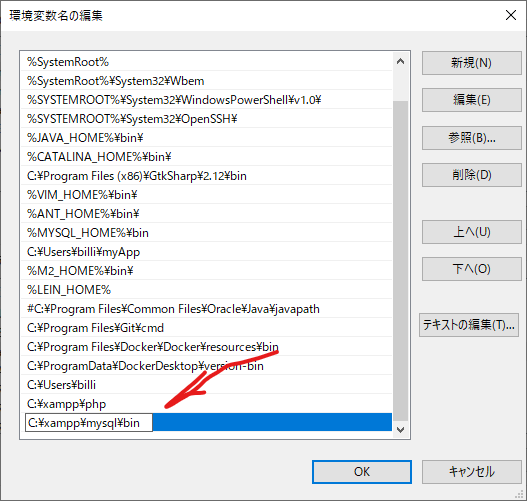
\includegraphics[width=13cm]{../06-mysql/01-mysql-path.png}
\vspace{3mm}

確認は、コマンドプロンプトを開きなおしてから、以下を入力する。

\begin{tcolorbox}
 $>$ mysql {-}{-}version
\end{tcolorbox}
\rightline{※ {-}{-} は ハイフン2つ}

mysql (MariaDB) のバージョンが表示される。


\end{document}

%% 修正時刻: Sat May  2 15:10:04 2020


%% 修正時刻: Fri 2024/09/27 09:15:021
